\documentclass[12pt]{article}

\usepackage{color}
\usepackage[portuguese]{babel}
\usepackage[utf8]{inputenc}
\usepackage{indentfirst}
\usepackage{graphicx}
\usepackage{verbatim}
\usepackage{listings}
\usepackage{url}
\usepackage{stringenc}
\usepackage{pdfescape}
\usepackage{subfig}
\usepackage{float}
\usepackage{eurosym}
\begin{document}

\setlength{\textwidth}{16cm}
\setlength{\textheight}{22cm}
\title{\huge\textbf{\textit{Android system for train tickets}}\linebreak
\Large\textbf{\\Trabalho \#1}\linebreak\linebreak\linebreak

\includegraphics[width=8cm]{feup.pdf}\linebreak \linebreak
\large{Mestrado Integrado em Engenharia Informática e Computação} \linebreak
\large{Computação Móvel \\ EIC0050-1S}\linebreak
}
\author{
Jose Rui Neto Faria - 201104362 (ei11046@fe.up.pt)\\
João Carlos Teixeira de Sá - 201107925 (ei11142@fe.up.pt)\\
Ricardo Daniel Soares da Silva - 201108043 (ei11079@fe.up.pt)\\
\\
\\ Faculdade de Engenharia da Universidade do Porto \\ Rua Roberto Frias, s\/n, 4200-465 Porto, Portugal
 \vspace{1cm}}
%\date{Junho de 2007}
\maketitle
\thispagestyle{empty}

%************************************************************************************************
%************************************************************************************************

\newpage

\tableofcontents

%************************************************************************************************
%************************************************************************************************

%*************************************************************************************************
%************************************************************************************************

\newpage

\section{Introdução}

O presente documento apresenta o desenvolvimento do projeto \textit{Android system for train tickets} para a unidade curricular de Computação Móvel.

O projeto tem como objetivo o desenvolvimento de um sistema, \textit{Android system for train tickets}, para uma empresa ferroviária capaz de ofereçer aos seus clientes uma aplicação Android através da qual estes possam consultar os horários disponíveis e comprar bilhetes. Os inspectores da empresa devem também ter acesso a uma aplicação Android onde possam validar os bilhetes para as viagens das quais estão encarregues.  

O sistema é composto por um servidor que é acedido tanto pela aplicação do cliente bem como pela do inspector sendo que, cada uma das aplicações apresenta um conjunto de pedidos distintos. O servidor encontra-se ligado a uma base de dados onde são armazenadas as informações relativas aos utilizadores do sistema, bilhetes, horários, entre outras.

A consulta dos horários pode ser efetuada por qualquer utilizador da aplicação, no entanto, a compra de bilhetes encontra-se restringida apenas a utilizadores registados no sistema. No momento de registo no sistema o utilizador deverá fornecer as informações relativas ao seu cartão de crédito uma vez que, este será o único método aceite para o pagamento dos bilhetes.


\section{Tecnologias}

O projeto foi desenvolvido usando o \textit{Android software development kit} para o desenvolvimento tanto da aplicação do clinte bem como do inspector tendo sido utilizadas a linguagem de programção Java com o auxílio de XML para o desenvolvimento dos \textit{layouts}. Relativamente ao servidor, foi desenvolvida uma aplicação web Node.js utilizando a linguagem de programação Javascript.

Adicionalmente foi utilizado para persistência de dados o sistema de gestão de base de dados \textit{SQLite} (tanto no servidor, como na aplicação do cliente).

Por último, para gestão de dependências do projeto foi usado o \textit{NuGet} e para gestão de versões foi utilizada a ferramenta \textit{Git} usando a plataforma \textit{GitHub}.


\section{Arquitetura}

\begin{figure}[h!]
    \centering
    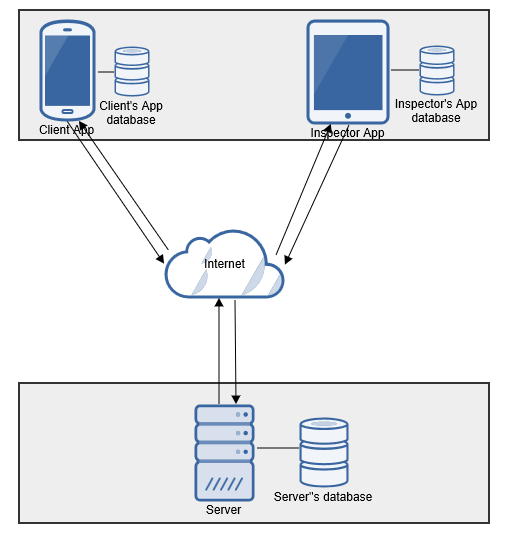
\includegraphics[width=0.8\textwidth]{arch.png}
    \caption{Arquitetura do Sistema.}
    \label{fig:arch}
\end{figure}

O sistema conta com duas aplicações Android, uma destinada aos clientes e outra destinada aos inspectores da empresa e um servidor capaz de responder aos pedidos de cada uma destas aplicações, como representado na fig. \ref{fig:arch}. Acrescenta-se ainda uma persistência de dados tanto no servidor bem como nas aplicações Android, ou seja, as aplicações apresentam também uma persistência de dados local.

\begin{figure}[h!]
	\centering
	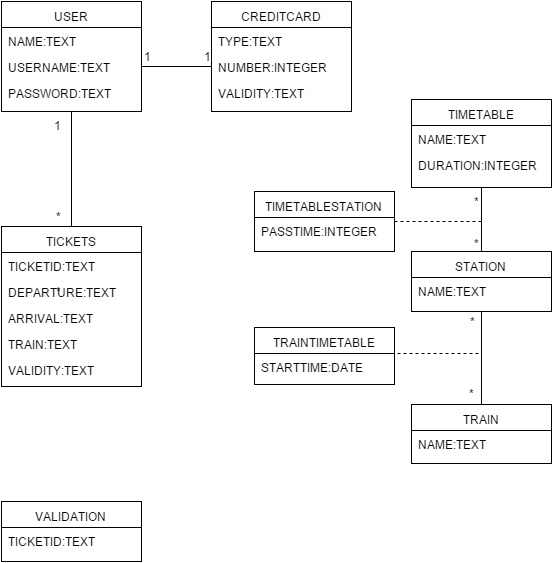
\includegraphics[width=0.8\textwidth]{db.png}
	\caption{Base de dados do servidor.}
	\label{fig:db}
\end{figure}

\newpage

Apresenta-se de seguida os componentes do sistema:
\begin{itemize}
\item Aplicação do cliente
\begin{itemize}
\item Aplicação Android destinada ao uso por parte dos clientes da empresa ferroviária e onde podem ser consultados os horários do comboio e fazer a compra de bilhetes. Esta aplicação comunica com o servidor sempre que existe uma ligação à Internet disponível contando também como uma base de dados local permitindo o uso de algumas funcionalidades mesmo sem essa ligação.
\end{itemize}
\item Aplicação do inspetor
\begin{itemize}
\item Aplicação Android destinada ao uso por parte dos inspectores da empresa ferroviária e onde podem ser validados os bilhetes dos clientes. Esta aplicação comunica com o servidor sempre que existe uma ligação à Internet disponível contando também como uma base de dados local permitindo a validação dos bilhetes mesmo sem essa ligação.
\end{itemize}
\item Servidor
\begin{itemize}
\item Aplicação com a lógica do sistema, transações e persistência de dados.
\item Disponibilização de uma API REST para consulta pelas aplicações do cliente e do inspector (cada uma das aplicações têm os seus pedidos bem definidos.).
\end{itemize}
\end{itemize}


\section{Front-end}

\subsection{Interface gráfica da aplicação do cliente}

\begin{figure}[H]
    \centering
    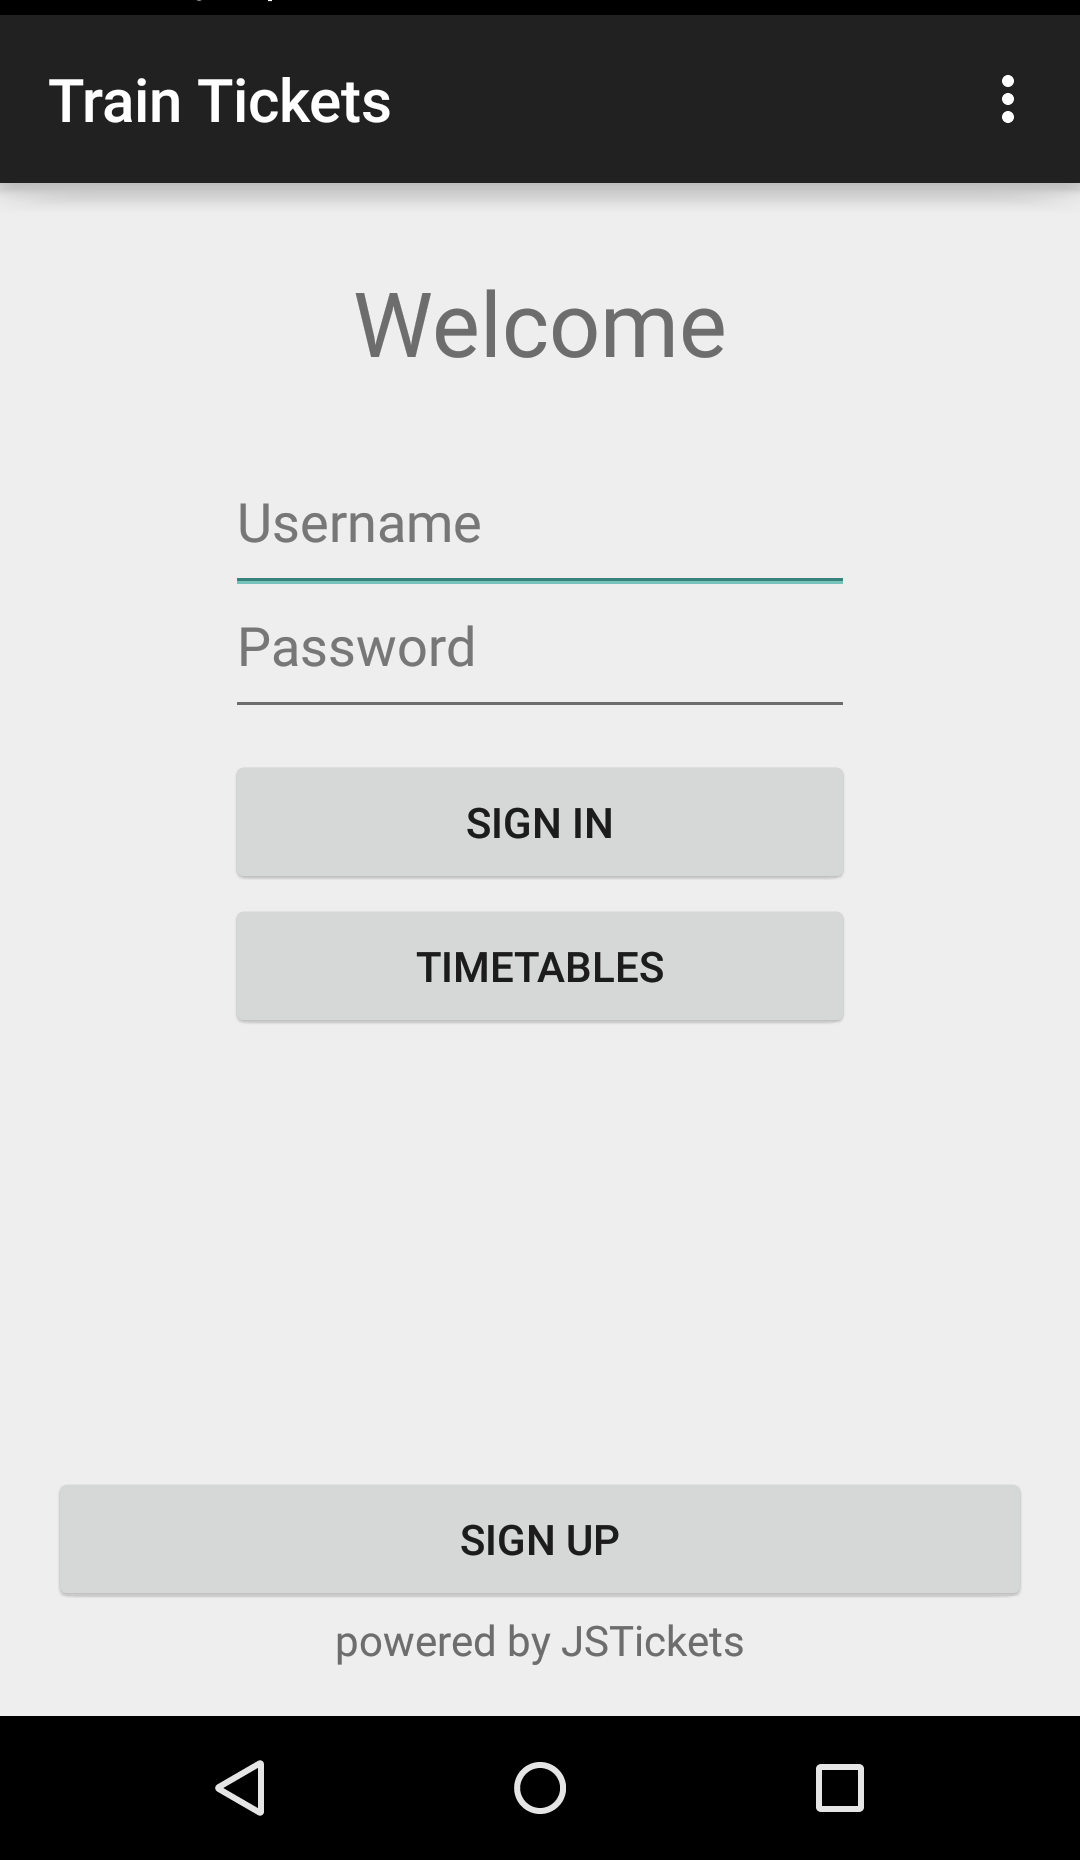
\includegraphics[width=0.5\textwidth]{Screenshot_Sign_In.png}
    \caption{Interface gráfica da aplicação do cliente - \textit{Sign In.}}
    \label{fig:c1}
\end{figure}

\begin{figure}[H]
	\centering
	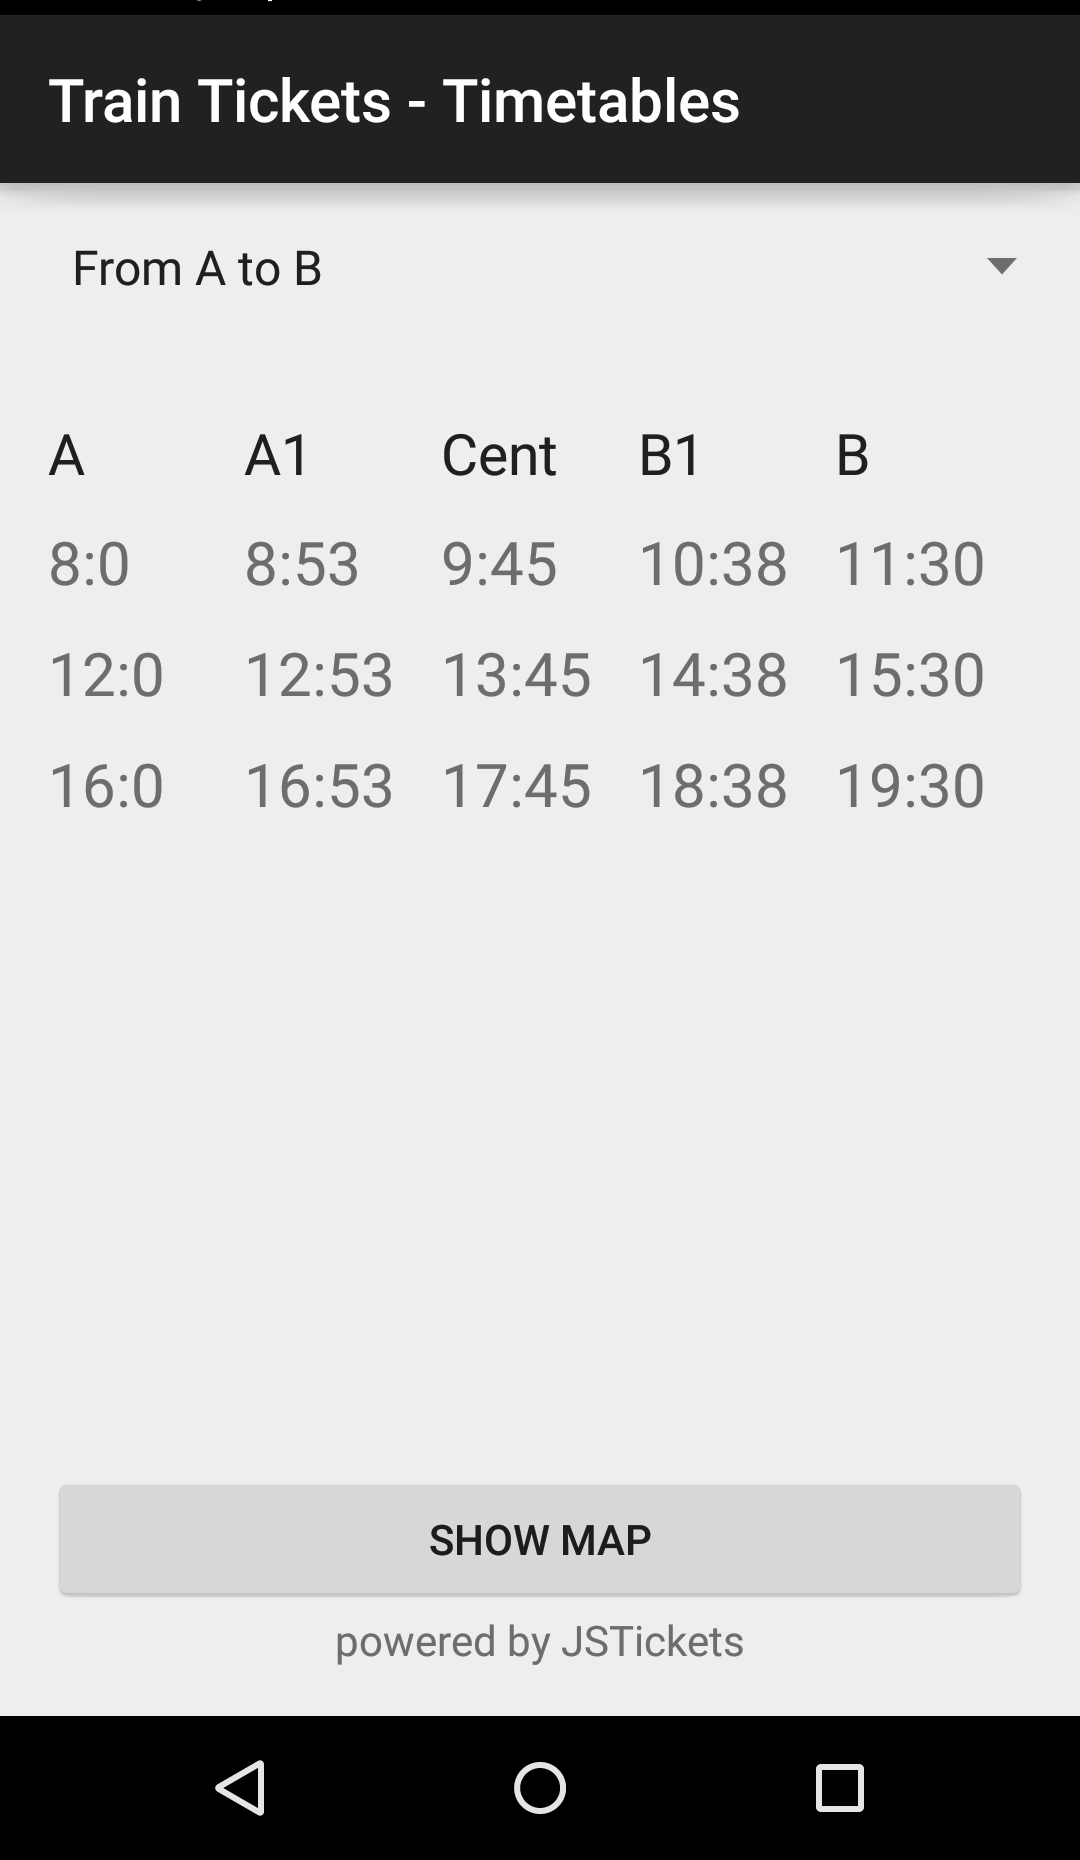
\includegraphics[width=0.5\textwidth]{Screenshot_Timetables.png}
	\caption{Interface gráfica da aplicação do cliente - Consulta de horários}
	\label{fig:c2}
\end{figure}

Ao nível da interface gráfica desenvolvida para a aplicação do cliente é disponibilizada numa primeira fase um ecrã de \textit{login}, fig. \ref{fig:c1}, onde o cliente pode entrar no sistema ou consultar os horários disponíveis, fig. \ref{fig:c2}.

Após o funcionário fazer \textit{login} no sistema são disponibilizadas as opções de comprar bilhetes, consultar os seus bilhetes ou ver os horários disponíveis, fig. \ref{fig:c3}, \ref{fig:c4} e \ref{fig:c5}.

Quando o utilizador seleciona um bilhete a partir do ecrã de consulta de bilhetes é apresentado um ecrã com a informação detalhada do bilhete selecionado, incluindo o QR associado, fig. \ref{fig:c6}.

\begin{figure}[H]
    \centering
    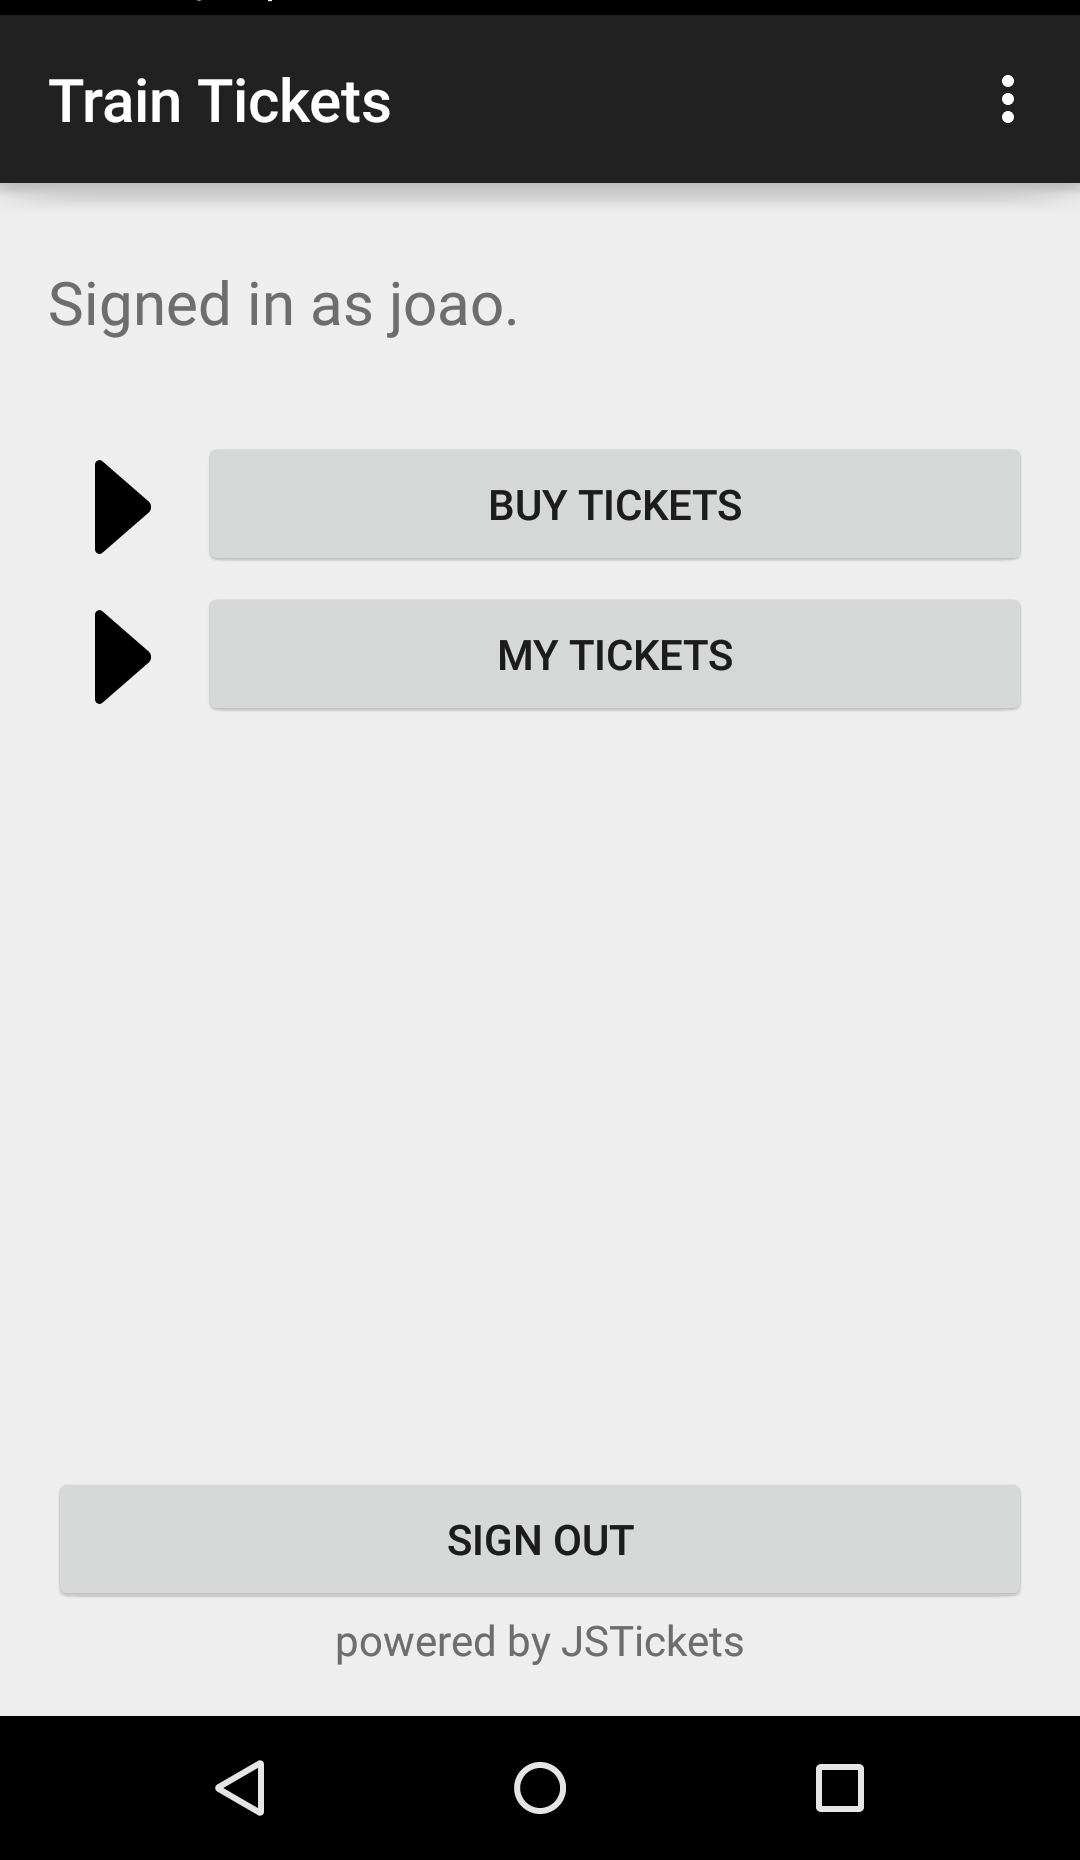
\includegraphics[width=0.5\textwidth]{Screenshot_Main.png}
    \caption{Interface gráfica da aplicação co cliente - Ecrã principal.}
    \label{fig:c3}
\end{figure}
\begin{figure}[H]
    \centering
    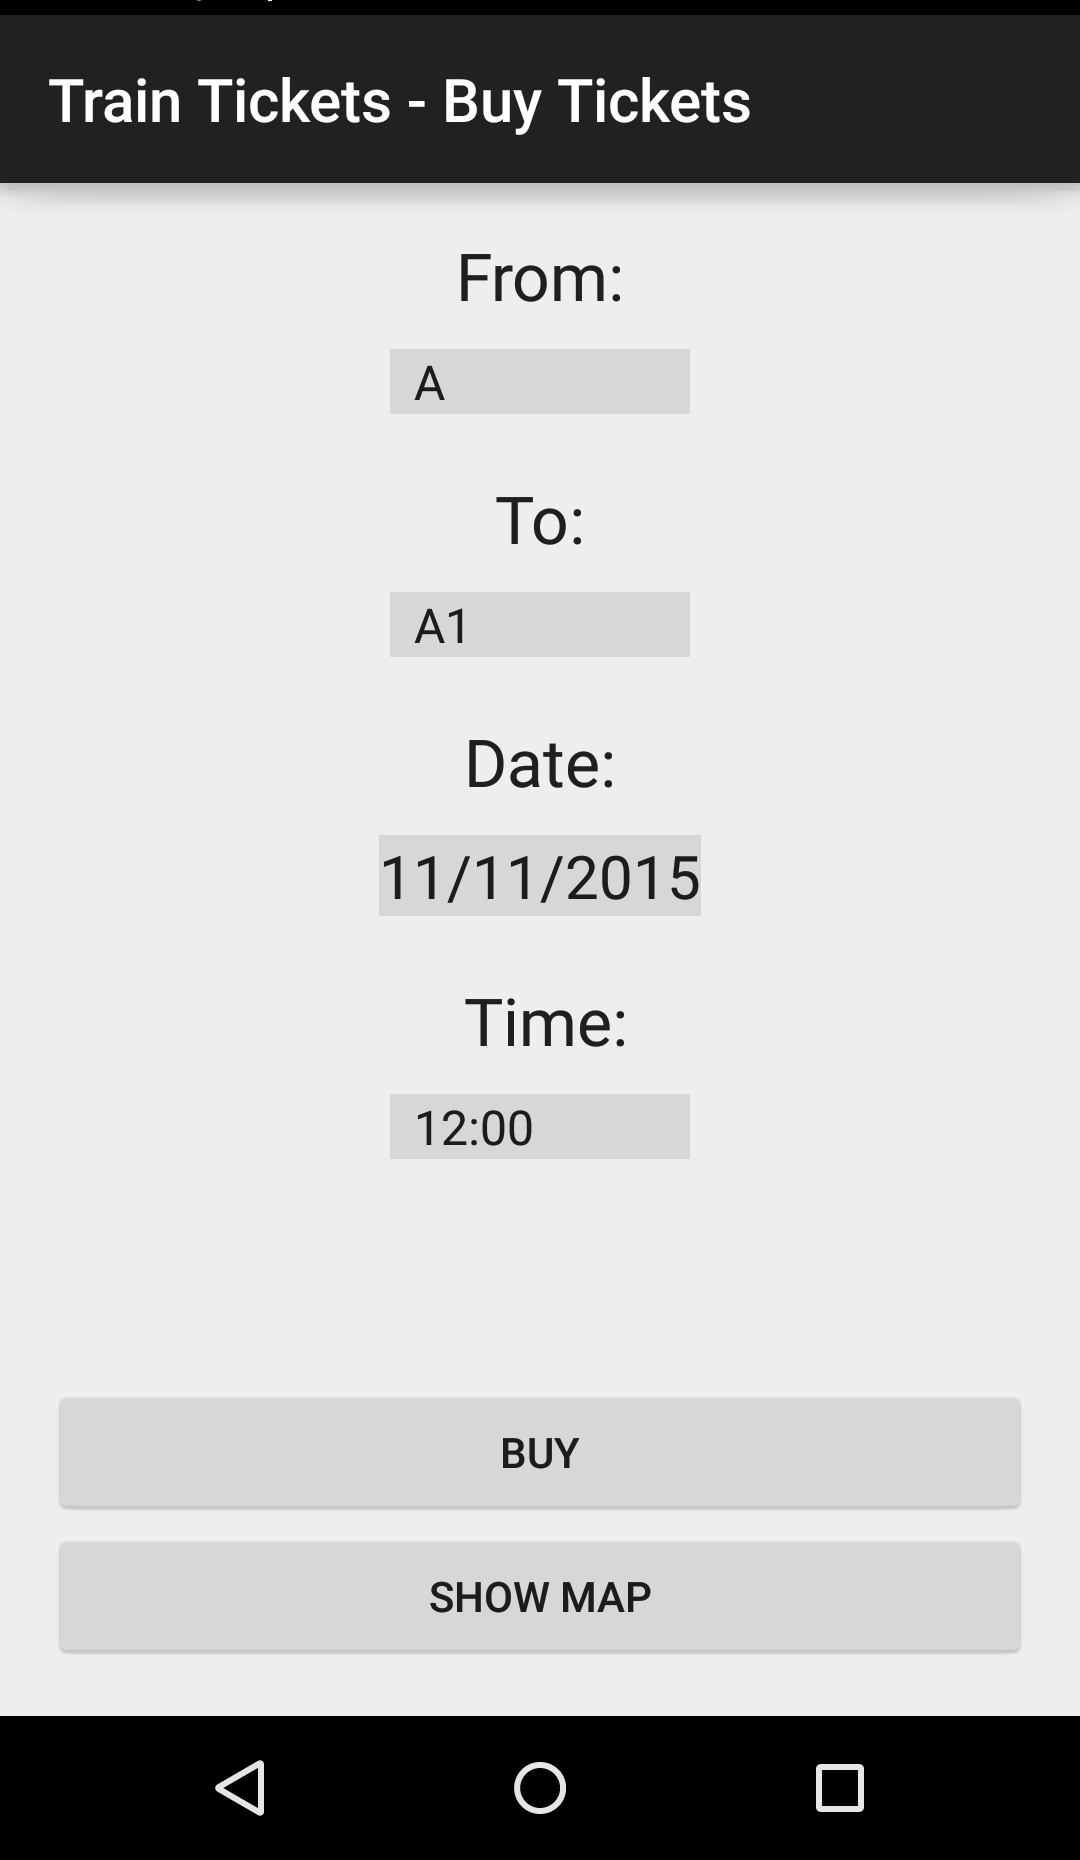
\includegraphics[width=0.5\textwidth]{Screenshot_Buy_Ticket.png}
    \caption{Interface gráfica da aplicação do cliente - Compra de bilhetes.}
    \label{fig:c4}
\end{figure}
\begin{figure}[H]
    \centering
    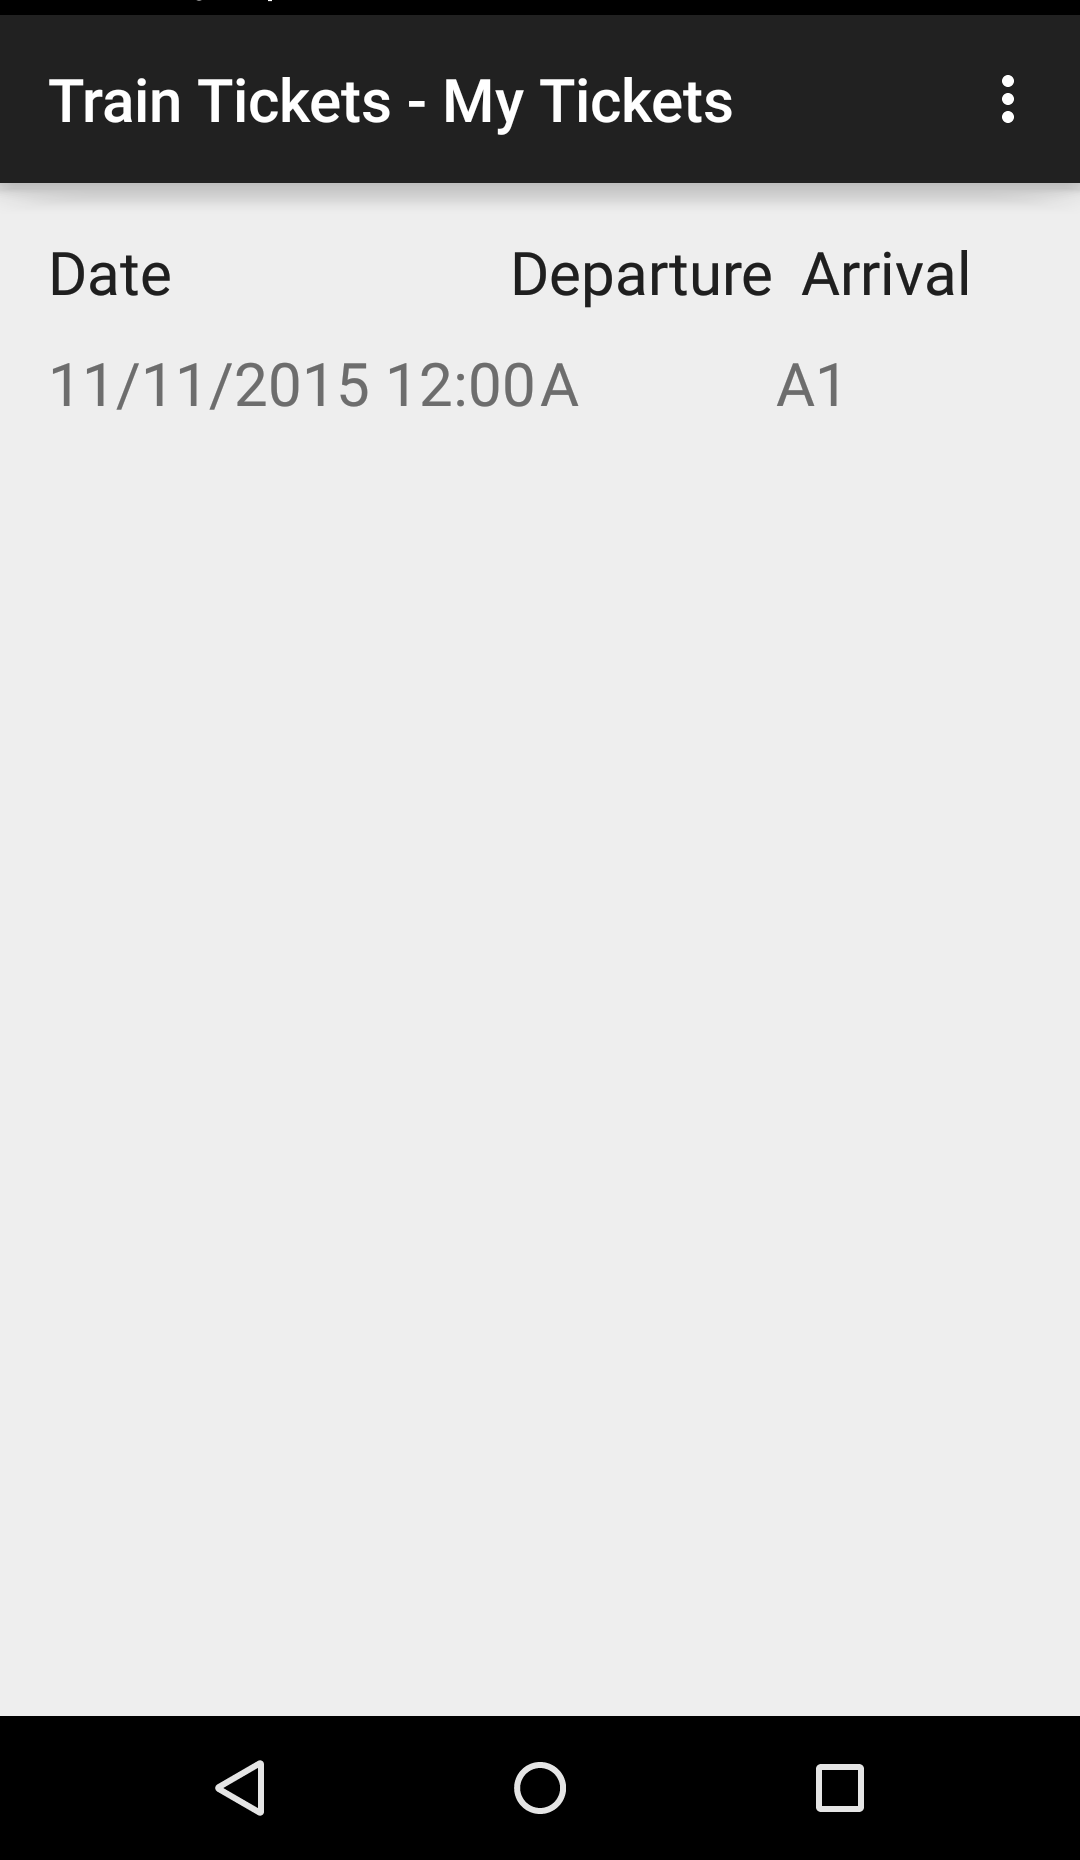
\includegraphics[width=0.5\textwidth]{Screenshot_My_Tickets.png}
    \caption{Interface gráfica da aplicação do cliente - Consulta de bilhetes.}
    \label{fig:c5}
\end{figure}
\begin{figure}[H]
	\centering
	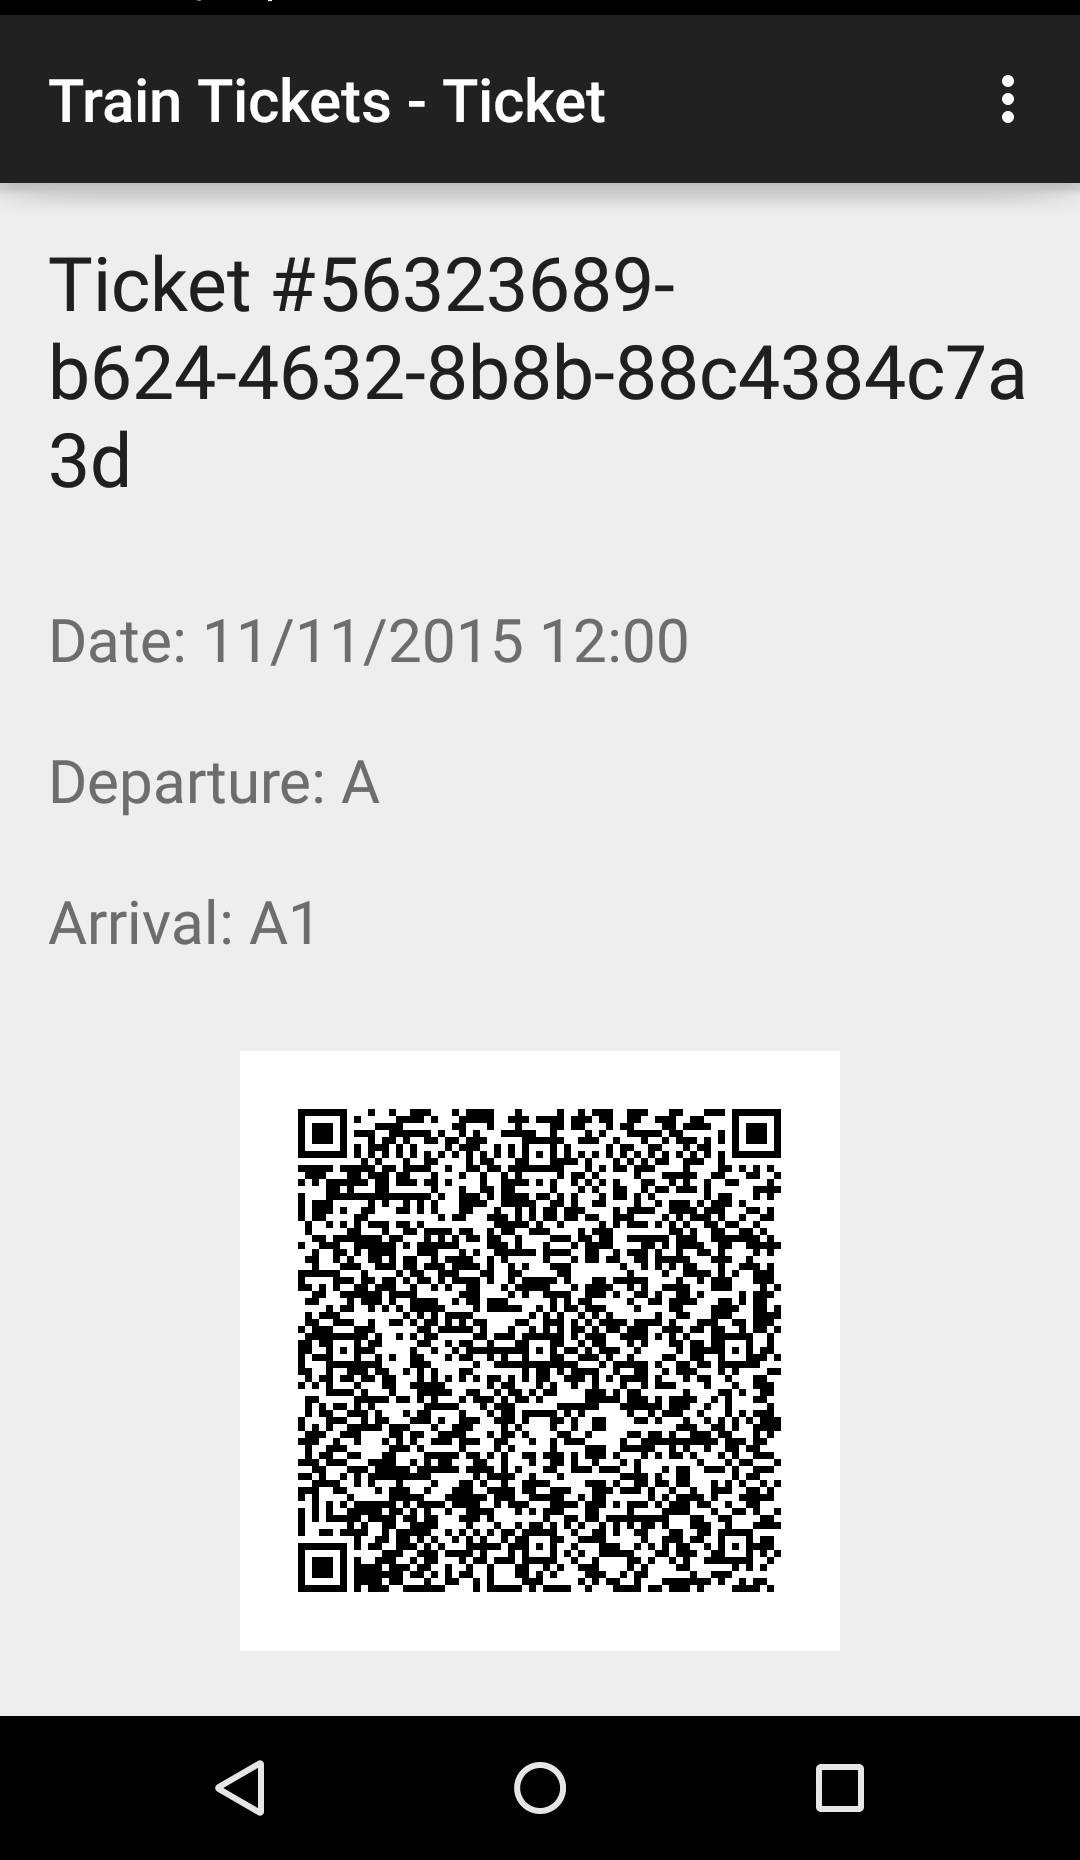
\includegraphics[width=0.5\textwidth]{Screenshot_Ticket.png}
	\caption{Interface gráfica da aplicação do cliente - Consulta de bilhete.}
	\label{fig:c6}
\end{figure}

\subsection{Interface gráfica da aplicação do inspector}

\begin{figure}[H]
    \centering
    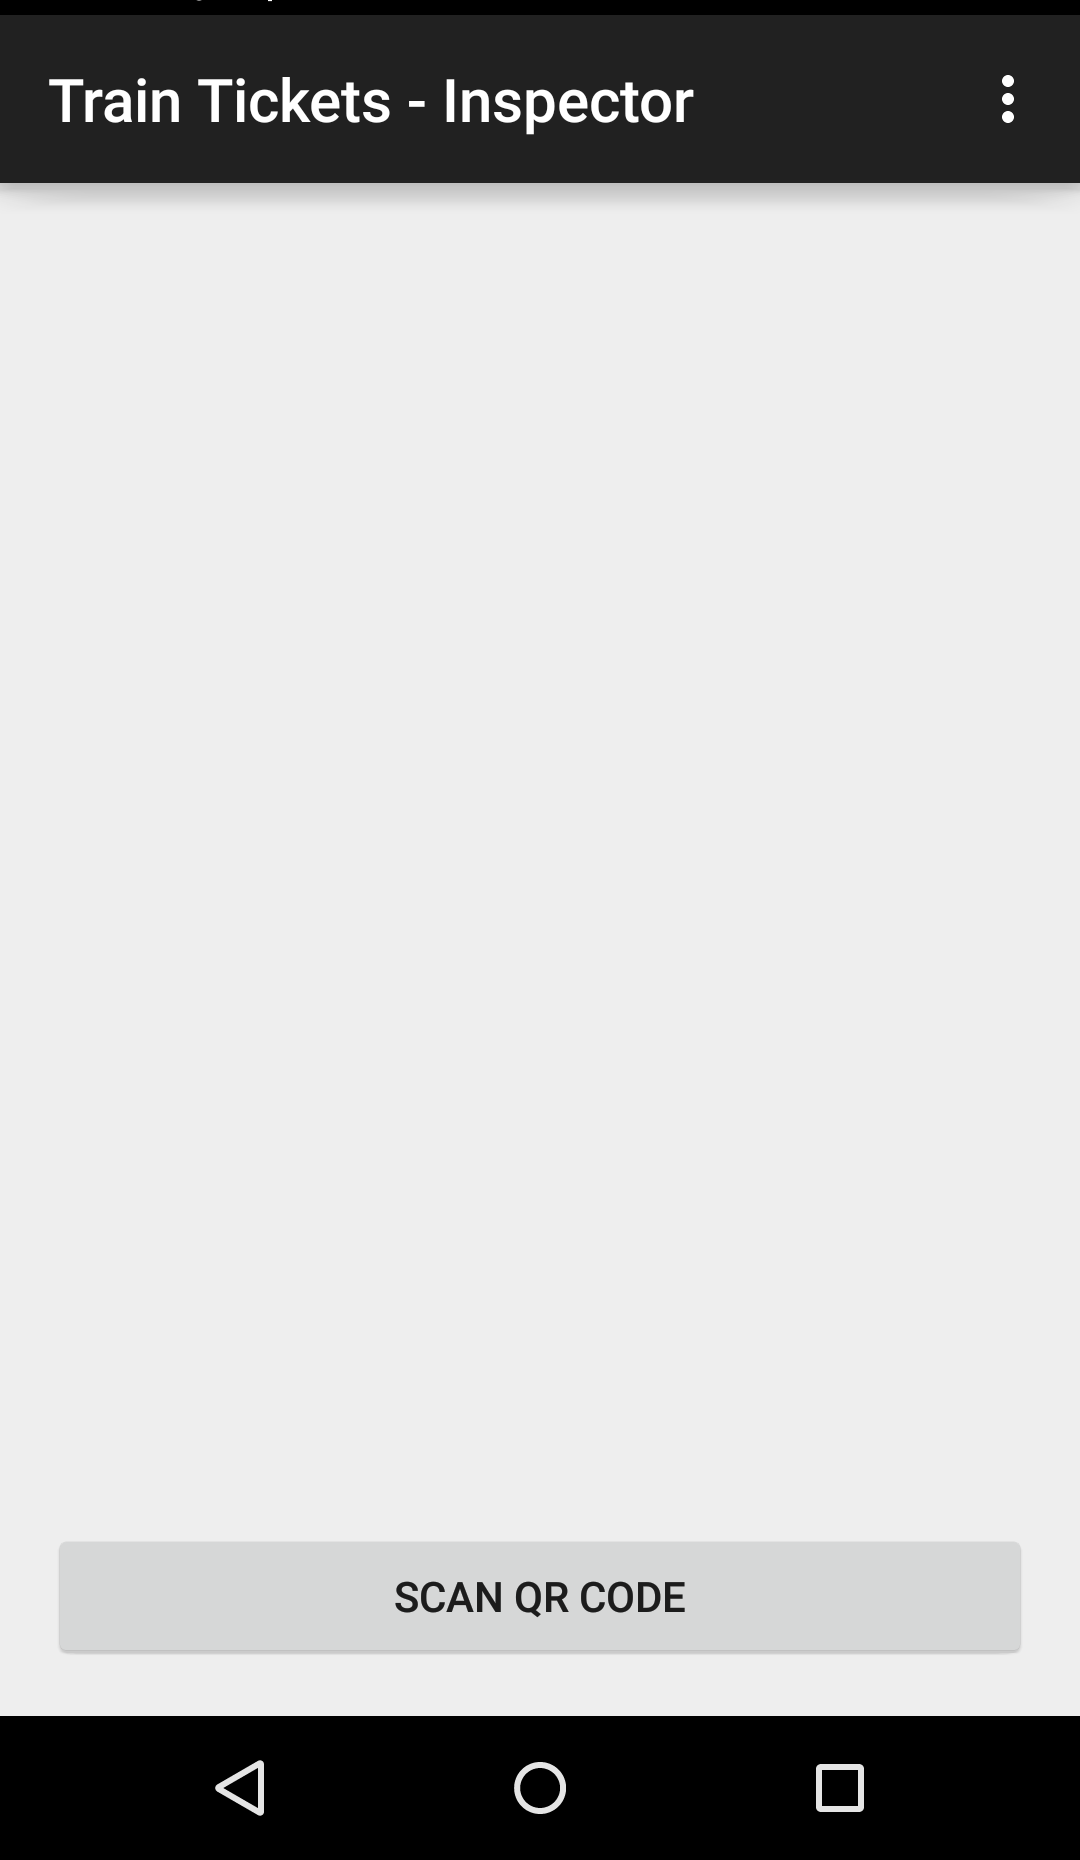
\includegraphics[width=0.5\textwidth]{Screenshot_Inspector_Main.png}
    \caption{Interface gráfica da aplicação do inspector - Ecrã principal.}
    \label{fig:c7}
\end{figure}

\begin{figure}[H]
	\centering
	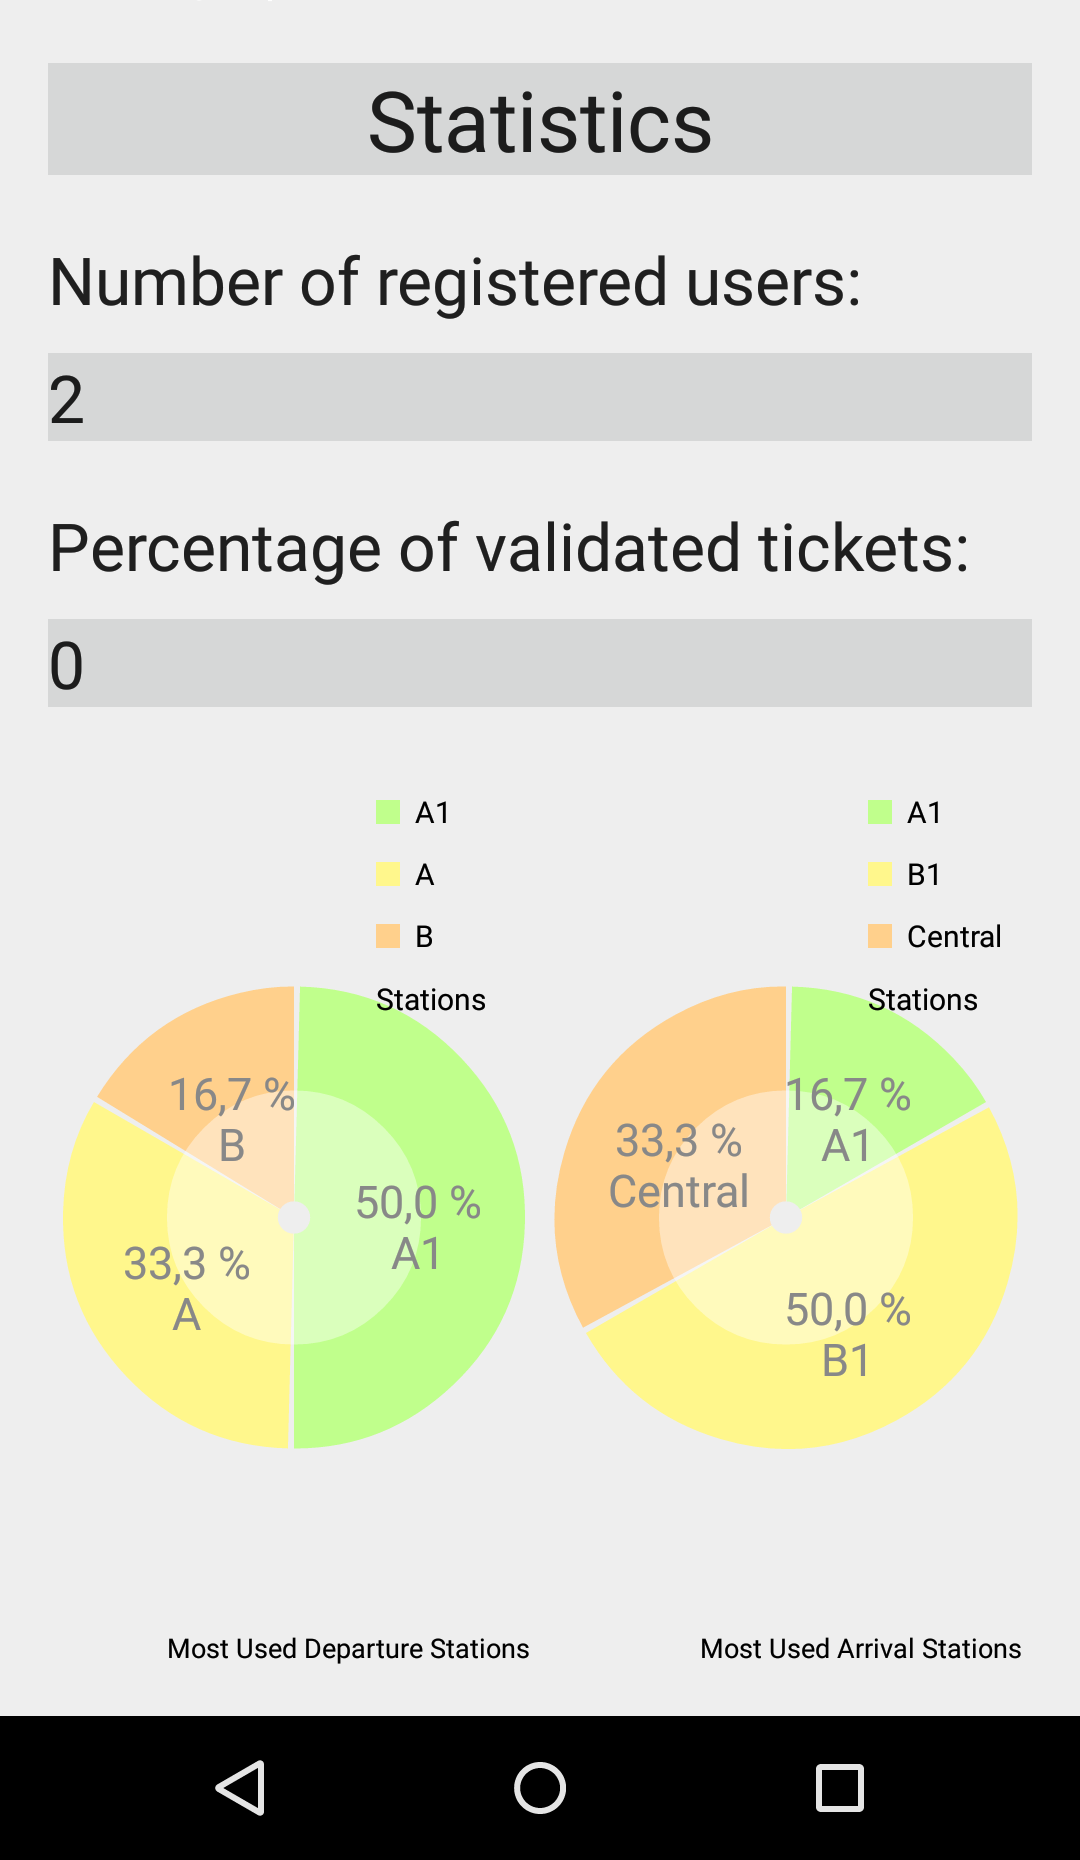
\includegraphics[width=0.5\textwidth]{Screenshot_Inspector_Statistics.png}
	\caption{Interface gráfica da aplicação do inspector - Estatísticas.}
	\label{fig:c8}
\end{figure}

Ao nível da interface gráfica desenvolvida para a aplicação do inspector é apresentado um ecrã inicial com um botão para proceder à validação de um bilhete através da leitura do respetivo código QR, fig. \ref{fig:c7}.

Ao carregar no menu de opções é também possível aceder a um ecrã onde são apresentados alguns dados estatísticos, \ref{fig:c8}.

\subsection{Casos de Uso}
\begin{figure}[H]
	\centering
	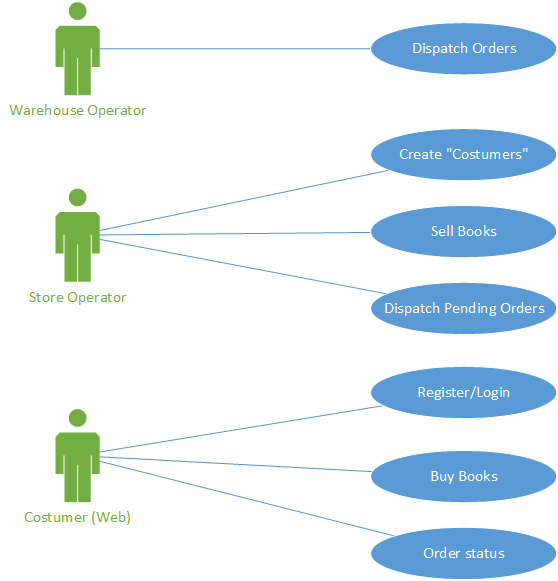
\includegraphics[width=0.6\textwidth]{use.png}
	\caption{Diagrama de casos de uso.}
	\label{fig:use}
\end{figure}


\section{Conclusão}

O sistema encontra-se desenvolvido com todas as funcionalidades solicitadas no enunciado do projeto, possibilitando aos clientes e aos inspectores da empresa ferroviária uma utilização total do sistema.

\subsection*{Testes}

Para testar o correto funcionamento do sistema foram efetuadas várias experiências tanto ao nível da aplicação do cliente como do inspector assim como, foram testados vários casos de falha ou do cliente e/ou servidor e garantida a persistência dos dados.

\subsection*{\textit{Deploy}}

O sistema pode ser utilizado colocando o servidor Node.js a correr, colocando o respetivo endereço IP do servidor nas configurações de ambas as aplicações e correndo-as posteriormente num dispositivo com o sistema operativo Android.

\subsection*{Credenciais \textit{Demo}}

Aplicação do cliente:
\begin{itemize}
	\item \textit{Username}: joao
	\item \textit{Password}: joao
\end{itemize}

\section{Recursos}

\subsection{Bibliografia}
\begin{description}
	\item Android API Guides, \url{https://developer.android.com/guide/index.html}.
	\item Distribution and Integration Technologies, Miguel Monteiro, Faculdade de Engenharia da Universidade do Porto, \url{https://web.fe.up.pt/~apm/CM/}.
\end{description}
\subsection{\it{Software}}
\begin{description}
	\item Android Studio, Google, \url{https://developer.android.com/sdk/index.html}.
	\item BlueStacks App Player, BlueStacks, \url{www.bluestacks.com/}.
	\item WebStorm, JetBrains, \url{https://www.jetbrains.com/webstorm/}.
	\item Sublime Text, \url{www.sublimetext.com/}.
	\item DB Browser for SQLite, \url{http://sqlitebrowser.org/}.
\end{description}


\end{document}
